\section{Billingsley Section 1}
[Berkeley 202a]
[Billingsley - Probability \& Measure]

Why does he say ``closed under countable unions and intersections.​''?

  Billingsley p.19:
  \begin{quote}
    ...require a collection that contains the intervals and is closed under countable unions and intersections.
    Note that a singleton $\{x\}$ is a countable intersection of intervals:
    \begin{align*}
      \bigcap_{n=1}^\infty \Big(x -\frac{1}{n}, x\Big] = \{x\}.
    \end{align*}
  \end{quote}


\begin{itemize}
\item $\Omega = [0, 1]$
\item $\om \in \Omega$
\item $d_n(\om) \in \{0, 1\} = $ $n$-th digit in binary expansion of $\om$
\item Rademacher function $r_n(\om) = 2d_n(\om) - 1 \in \{-1, 1\}$
\end{itemize}

\subsection{Weak Law of Large Numbers}

Define the partial sum $s_n(\om) = \sum_{i=1}^n r_i(\om)$, i.e. the number of $1$s minus the number of $0$s in
the first $n$ digits of the binary expansion of $\om$. (The displacement of the random walk after $n$ steps.)

\begin{lemma}
  \begin{align*}
    \int_0^1 s_n(\om)^2 \d\om = n
  \end{align*}
\end{lemma}

I.e., viewed as a sequence of $n$ coin tosses yielding $-1$ or $+1$, the variance (expected squared distance
from mean) of their sum is $n$.

\begin{proof}
  Note that $s_n(\om)^2 = \sum_{i=1}^n r_i(\om)^2 - 2\sum_{i<j}r_i(\om)r_j(\om)$. Integrating over $[0, 1]$ we have
  \begin{align*}
    \int_0^1 s_n(\om)^2 \d\om
    &= \sum_{i=1}^n \int_0^1 r_i(\om)^2 \d\om - 2\sum_{i<j}\int_0^1r_i(\om)r_j(\om) \d\om \\
    &= \sum_{i=1}^n \int_0^1 1 \d\om - 0 \\
    &= n.
  \end{align*}
  We used there the fact that $\int_0^1r_i(\om)r_j(\om) \d\om = 0$ for $i < j$, i.e that the Rademacher
  functions are orthogonal. An argument for this is that as we move through a rank $i$ dyadic
  interval, $r_i(\omega)$ is constant (either $-1$ or $+1$) while at rank $j$ below, $r_j(\omega)$ flickers
  between $-1$ and $+1$, spending an equal amount of time in each.
\end{proof}


\begin{lemma}[Markov's Inequality]
  Let $f: [0, 1] \to \R^+$ be a step function. Then
  \begin{align*}
    P\Big(\Big\{x: f(x) \geq \alpha\Big\}\Big) \leq \frac{1}{\alpha}\int_0^1 f(x) \dx.
  \end{align*}
\end{lemma}




\begin{intuition}
  Think of the statement in rearranged form:
  \begin{align*}
    \alpha P\Big(\Big\{x: f(x) \geq \alpha\Big\}\Big) \leq \int_0^1 f(x) \dx.
  \end{align*}



  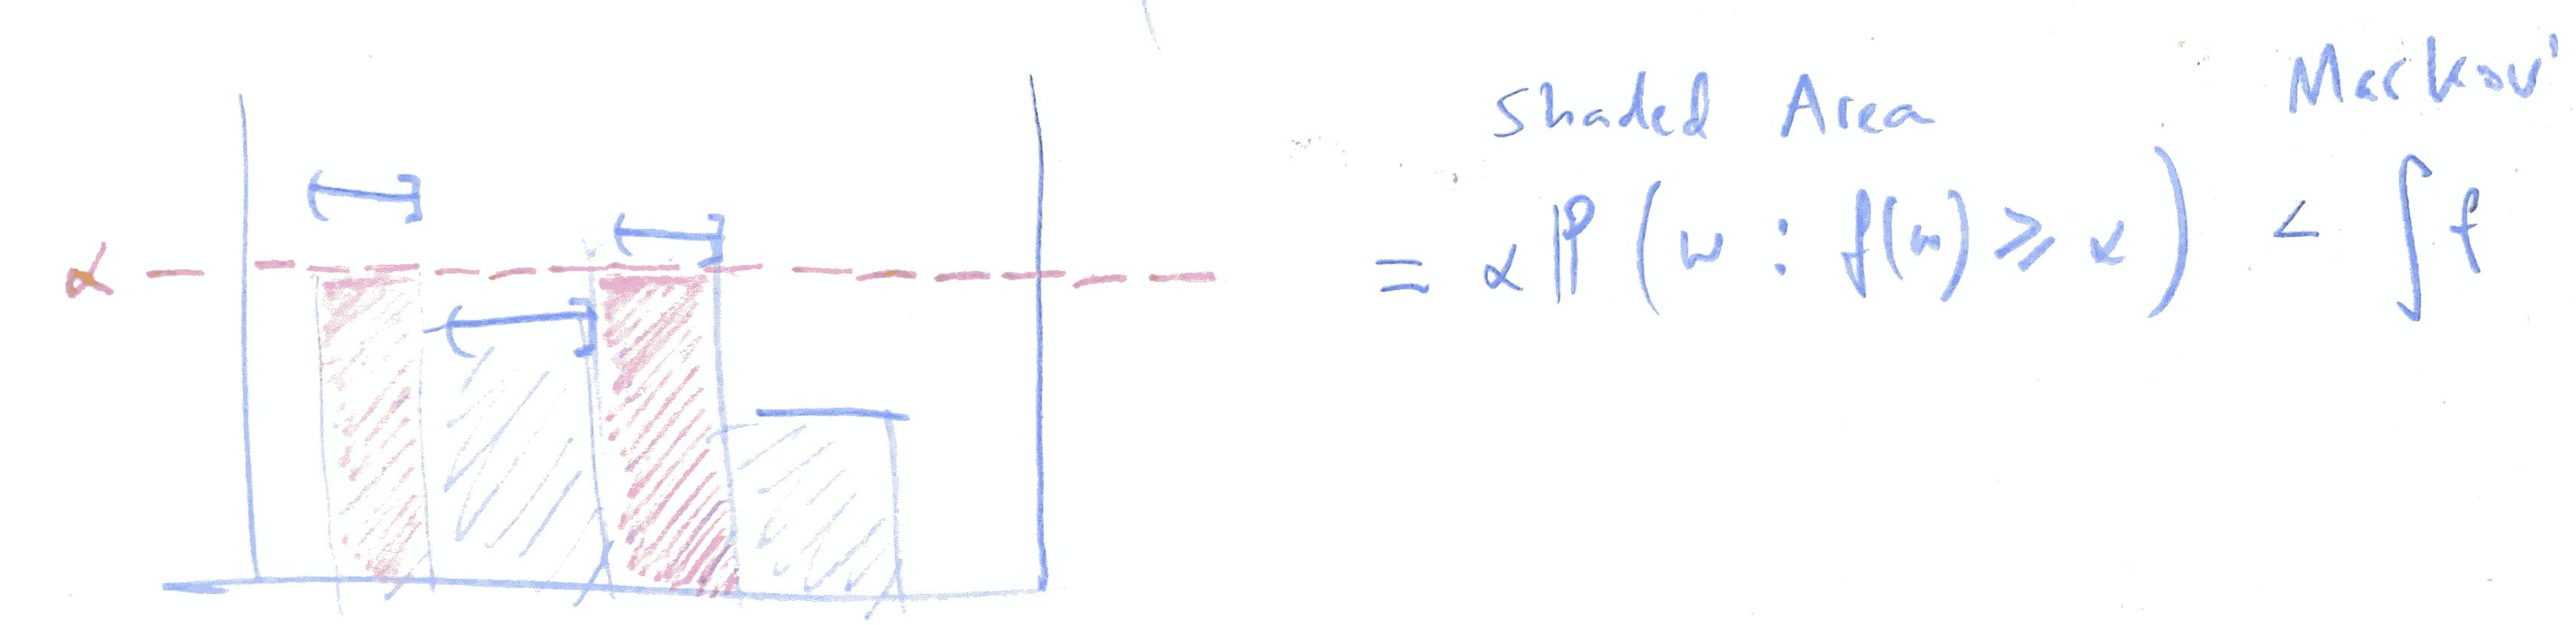
\includegraphics[width=400pt]{img/analysis--real-analysis--measure-theory--weak-law-of-large-numbers-c9c2.png}

  If $X \sim \Unif(0, 1)$ then the RHS is $\E[X]$.

\end{intuition}


\begin{proof}
  [me]

  Clearly
  \begin{align*}
    \int_{f(x) \geq \alpha} f \leq \int_{[0, 1]} f.
  \end{align*}
  Therefore
  \begin{align*}
    \int_{f(x) \geq \alpha} \alpha \leq \int_{[0, 1]} f
  \end{align*},
  or equivalently
\begin{align*}
  \alpha \int \textbf{1}_{f(x) \geq \alpha} \leq \int_{[0, 1]} f,
\end{align*}
which is the same thing as
  \begin{align*}
    \alpha P\Big(\Big\{x: f(x) \geq \alpha\Big\}\Big) < \int_0^1 f(x) \dx.
  \end{align*}
\end{proof}

\begin{theorem}[Weak Law of Large Numbers]
  Fix an $\epsilon > 0$. Then
  \begin{align*}
    \lim_{n \to \infty}P\Big(\Big\{\om: \frac{1}{n}\big|\sum_{i=1}^n r_i(\om)\big| \geq \epsilon\Big\}\Big) = 0.
  \end{align*}
\end{theorem}

In other words: we move through all the $\om \in [0, 1]$. For a given $\om \in [0, 1]$, compare the number
of $0$s and $1$s in the first $n$ digits of the binary expansion, and record the excess as a proportion of $n$;
this is $\frac{1}{n}|s_n(\om)|$. The theorem states that for all $\epsilon > 0$ the probability measure
associated with the set of $\om$s for which $\frac{1}{n}|s_n(\om)| > \epsilon$ goes to $0$ as $n \to \infty$.

\begin{proof}
  Fix an $\epsilon > 0$. We square both sides of the inequality, instead of working with the absolute value. So
  what we want to show is that $P\big(\big\{\om: s_n^2(\om) \geq n^2\epsilon^2\big\}\big) \to 0$
  as $n \to \infty$.

  It would be nice to find an expression for this probability measure as a function of $n$. However, what we'll
  do is find an upper bound: that will suffice also.

  Note that $s_n(\om)$ is a step function (and so $s_n^2(\om)$ is also):

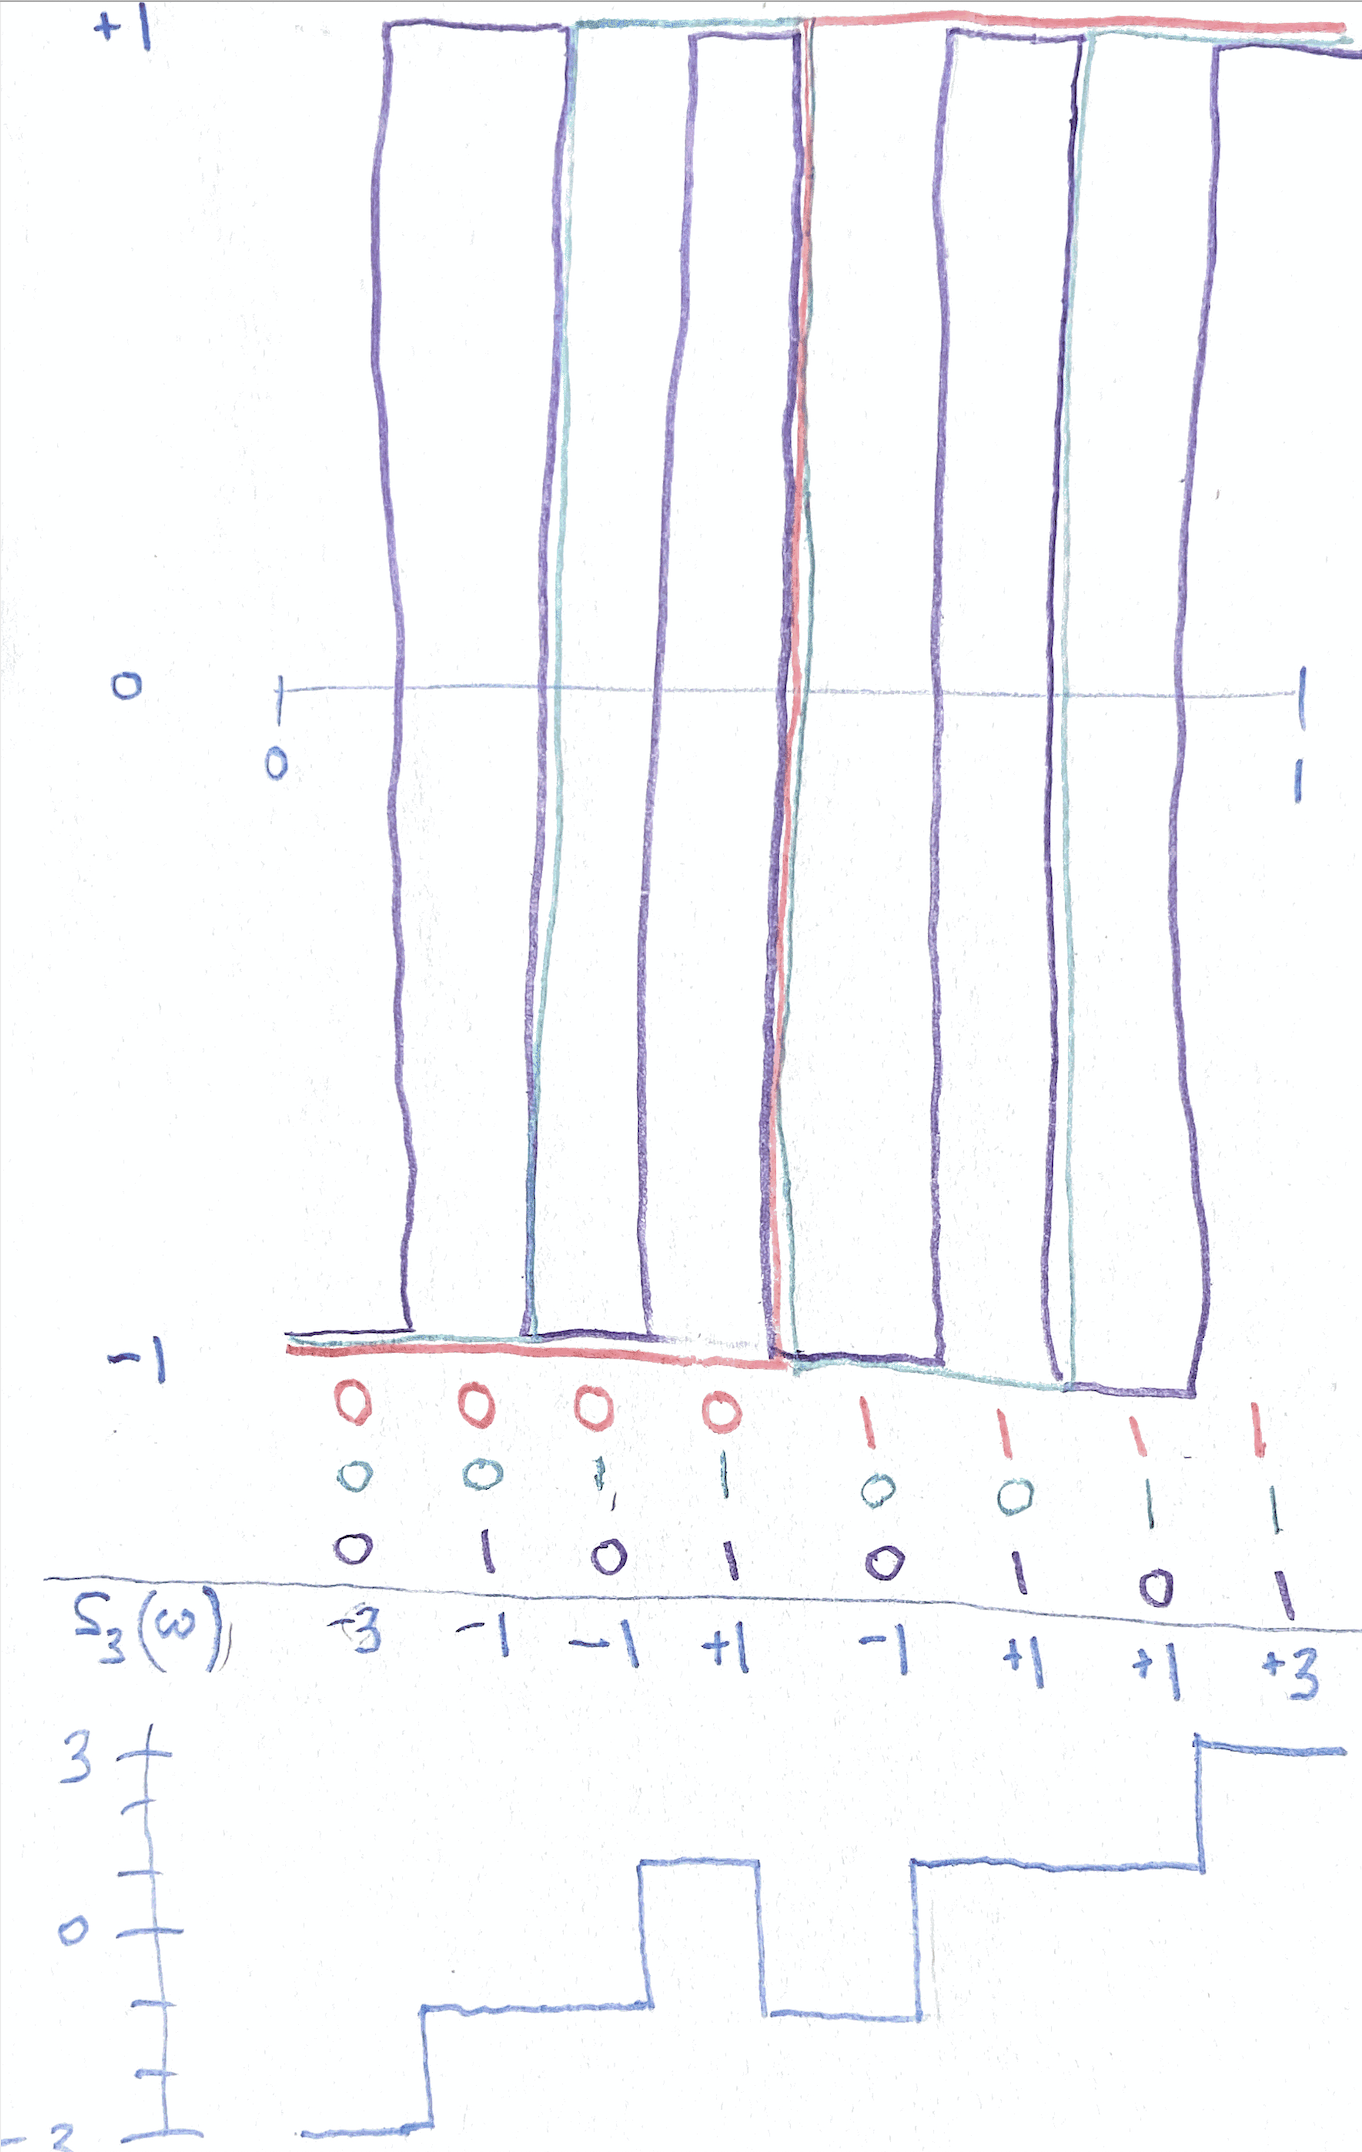
\includegraphics[width=200pt]{img/analysis--real-analysis--measure-theory--weak-law-of-large-numbers-c049.png}


By Markov's inequality / ``Shaded Area lemma​'' we have
\begin{align*}
  n^2\epsilon^2P\Big(\Big\{\om: s_n^2(\om) \geq n^2\epsilon^2\Big\}\Big) \leq \int_0^1 s_n^2(\om) \d\om = n
\end{align*}
and therefore
\begin{align*}
  P\Big(\Big\{\om: s_n^2(\om) \geq n^2\epsilon^2\Big\}\Big) \leq  \frac{1}{n\epsilon^2},
\end{align*}
which proves the desired result since it shows that the probability measure is bounded above by a quantity that
goes to $0$ as $n \to \infty$.
\end{proof}

\subsection{Strong Law of Large Numbers}

\red{TODO} Relation of Borel's normal number theorem to SLNN.

\begin{definition}[negligible, null set]
  A set $A$ is \defn{negligible} if, for any $\epsilon > 0$, it can be covered by a finite or countable
  union $\bigcup_k I_k$ of intervals with $\sum_k |I_k| < \epsilon$.
\end{definition}

Recall the weak law of large numbers:
  \begin{align*}
    \lim_{n \to \infty}P\Big(\Big\{\om: \frac{1}{n}\big|s_n(\om)\big| \geq \epsilon\Big\}\Big) = 0.
  \end{align*}

\begin{definition}[Normal numbers]
  Define the set of \defn{normal numbers} to be
  \begin{align*}
    N = \Big\{\om ~:~ \lim_{n\to\infty} \frac{1}{n}s_n(\om) = 0 \Big\}.
  \end{align*}
\end{definition}

\begin{theorem*}[Borel's normal number theorem]
  $N^c = \R \setminus N$ is negligible.
\end{theorem*}

\begin{intuition}
  Note that the set of normal $\om$ can be written as the set of $\om$ that

  ``eventually stay within $1$​'' AND
  ``eventually stay within $1/2$'' AND
  ``eventually stay within $1/3$'' AND
  ``eventually stay within $1/4$'' ...
  \begin{align*}
    N = \bigcap_{k=1}^\infty \bigcup_{m=1}^\infty\bigcap_{n \geq m} \big\{ \om ~:~ \big|\frac{1}{n}S_n(\om)\big| < \frac{1}{k} \big\}.
  \end{align*}

  Visualize the $s_n$ sequence of a non-normal number $\om$, stretching off to infinity. However far we’ve
  gone, there will always be another point further along at which an excursion of the random walk sticks out
  further than $\eps$. But despite the fact that this must always happen, it’s less and less likely the further
  we go. The fact that it must always happen again corresponds to the fact that we can write the event as a
  countable union: (happened by this generation) union with (happened at the next generation), etc. But at the
  same time, since it’s getting harder and harder, for any given $\gamma >0$ we can find some generation $m$
  beyond which the union sums to less than $\gamma$. nevertheless , the event is equal to the union beyond that
  point, since the departures must always keep occurring (otherwise the number would be normal). So the union
  doesn’t have to include earlier generations.

  This is why the complement of the normal numbers is negligible. Perhaps it’s typical of negligible sets that
  they correspond to an event that must always occur one more time, and yet get ever less and less likely?
\end{intuition}

\begin{proof}
  Let $(\eps_n)$ be a sequence that converges to zero, and define a sequence of sets $(A_n)$, where
  \begin{align*}
    A_n = \Big\{\om : \Big|\frac{1}{n} s_n(\om)\Big| \geq \eps_n\Big\}.
  \end{align*}
  (We can think of $A_n$ as the set of $\om$ whose binary expansions are ``not normal so far​''.)

  Note that, for any given $m$, we have the following: a number that stays inside $\eps_n$ for ever is normal:
  \begin{align*}
    \Big(\bigcap_{n=m}^\infty A_n^c\Big) \subset N.
  \end{align*}
  Equivalently, a non-normal number must stray outside $\eps_n$ at some point:
  \begin{align*}
    N^c \subset \Big(\bigcup_{n=m}^\infty A_n\Big).
  \end{align*}
  Recall that our aim is to cover $N^c$ with a countable union of intervals, where the total length of the
  intervals is arbitrarily small (an ``efficent covering​​''). If we can show that the $A_n$ meet that
  description then we are done.

  Recall that $s_n$ is a step function such that, if $\om \in A_n$ then $\om' \in A_n$ for every $\om'$ in the
  same rank-$n$ dyadic interval as $\om$. Therefore each set $A_n$ is a finite disjoint
  union $\bigcup_{k}I_{nk}$ of intervals, and $P(A_n) = \sum_k |I_{nk}|$.

  So what we need to do is show that, for any given $\gamma > 0$, there exists a sequence $(\eps_n)$ converging
  to zero, and an $m$, such that $\sum_{n=m}^\infty P(A_n) < \gamma$.

  At this point, we need to find an expression for an upper bound on $P(A_n)$ in terms of $n$ and $\eps_n$.
  From the lemma, we have
  \begin{align*}
    P(A_n) \leq \frac{3}{n^2\eps_n^4},
  \end{align*}
  so we would like to find $(\eps_n)$ and $m$ such that
  \begin{align*}
    \sum_{n=m}^\infty \frac{3}{n^2\eps_n^4} < \gamma.
  \end{align*}
  To do so, we need only choose $(\eps_n)$ so that the series $\sum_nn^{-2}\eps_n^{-4}$
  converges: $\eps_n = n^{-1/8}$ will do. Then, since the series converges, there exists an $m$ such that the
  tail sums to less than $\gamma$, as required.
\end{proof}

\begin{lemma}
  Let $A_n = \Big\{\om : \Big|\frac{1}{n} s_n(\om)\Big| \geq \eps\Big\}$.

  For all $n \in \N$, we have (by taking the 4th power of both sides of the inequality and applying Markov's
  inequality)
  \begin{align*}
    P(A_n) \leq \frac{1}{n^4\eps^4} \int_0^1 s_n^4(\om) \d\om,
  \end{align*}
  and (by considering integrals of products of four Rademacher functions)
  \begin{align*}
    \int_0^1 s_n^4(\om) \d\om \leq 3n^2.
  \end{align*}
  Therefore
  \begin{align*}
    P(A_n) \leq \frac{3}{n^2\eps^4}.
  \end{align*}
\end{lemma}

\newpage
\subsection{An interval of  positive length is not negligible}

\begin{definition*}[length of an interval]
  The \defn{length} of $(a, b)$ is $|(a, b)| = b - a$.
\end{definition*}

\begin{theorem*}
  Let $I$ be an interval of positive length and let $I_1, I_2, \ldots$ be intervals.
  \begin{enumerate}
  \item If $\bigcup_k I_k \subseteq I$ (disjoint) then $\sum_k |I_k| \leq |I|$
  \item If $\bigcup_k I_k \supseteq I$ then $\sum_k |I_k| \geq |I|$. I.e. no cover of $I$ is negligible.
  \end{enumerate}
  A corollary is that if $\bigcup_k I_k = I$ then $\sum_k |I_k| = |I|$.
\end{theorem*}

\begin{proof}
  Let $I = (a, b)$ and let $I_k = (a_k, b_k)$ for all $k$.

  First, we show that if $\bigcup_k I_k \subseteq I$ (with the $I_k$ disjoint) then $\sum_k |I_k| \leq |I|$.

  There are two cases:
  \begin{enumerate}
  \item {\bf Finite cover}:

    The claim is that for any collection of $n$ disjoint intervals, if $\bigcup_{k=1}^n I_k \subseteq I$
    then $\sum_{k=1}^n |I_k| \leq |I|$.

    This is clearly true for a collection of intervals of size $n = 1$.

    Assume it's true for any collection of intervals of size $n-1$, and consider a collection of $n$ disjoint
    intervals with $\bigcup_{k=1}^n I_k \subseteq I$.

    Label the intervals $I_1, \ldots, I_n$, sorted by their left endpoint in ascending order. Note that the
    union of the first $n-1$ intervals is contained within $(a, a_n)$ and that the $n$-th interval has
    length $b_n - a_n \leq b - a_n$. Thus we have
    \begin{align*}
      \sum_{k=1}^n |I_k|
      &= \sum_{k=1}^{n-1}|I_k| + |I_n| \\
      &\leq (a_n - a) + (b - a_n) \\
      &= b - a.
    \end{align*}
    Therefore it is true for all $n$ by induction.

  \item {\bf Infinite cover}:

    The claim is that for any countably infinite collection of $n$ disjoint intervals,
    if $\bigcup_{k=1}^\infty I_k \subseteq I$ then $\sum_{k=1}^\infty |I_k| \leq |I|$.

    Consider an infinite collection of intervals satisfying $\bigcup_{k=1}^\infty I_k \subseteq I$.

    Note that for every finite subcollection of size $n$ we have $\sum_{k=1}^n |I_k| \leq |I|$ by the finite case.

    Therefore $\sum_{k=1}^\infty |I_k| = \sup \sum_{k=1}^n |I_k| \leq |I|$ where the supremum is over the set
    of all finite subcollections. Since this set is non-empty, the supremum is a finite positive number.
  \end{enumerate}
  ~\\~\\
  Finally, we show that if $\bigcup_k I_k \supseteq I$ then $\sum_k |I_k| \geq |I|$.
  Again, there are two cases:
  \begin{enumerate}
  \item {\bf Finite cover}:

    The claim is that for any collection of $n$ intervals, if $\bigcup_{k=1}^n I_k \supseteq I$
    then $\sum_{k=1}^n |I_k| \geq |I|$.

    In other words, that the total length of a finite cover of $I$ is bounded below by $|I| > 0$.

    Again, it's obvious for a cover comprising a single interval ($n=1$).

    Assume it's true for any cover comprising $n-1$ intervals, and consider a cover comprising $n$ intervals.

    Again, label the intervals $I_1, \ldots, I_n$, sorted by their left endpoint in ascending order.

    Note that the first $n-1$ intervals cover the interval $(a, b_{n-1})$ and that $|I_n| \geq b - b_{n-1}$.
    Thus we have
    \begin{align*}
      \sum_{k=1}^n |I_k|
      &= \sum_{k=1}^{n-1}|I_k| + |I_n| \\
      &\geq (b_{n-1} - a) + (b - b_{n-1}) \\
      &= b - a.
    \end{align*}

  \item {\bf Infinite cover}\\

    The claim is that for any infinite cover $\bigcup_{k=1}^\infty I_k \supseteq I$ we have $\sum_{k=1}^\infty |I_k| \geq |I|$.

    Consider a countably infinite cover of $I$.

    We might think that we could make an argument analogous to the one above:

    Note that for every finite subcover of size $n$ we have $\sum_{k=1}^n |I_k| \geq |I|$.

    Therefore $\sum_{k=1}^\infty |I_k| = \inf \sum_{k=1}^n |I_k|  \geq |I|$ where the infimum is over the set of all finite subcovers.

    However, we have to show that a finite subcover exists; otherwise the infimum would be $+\infty$.

    So what we do is construct a closed interval $[a + \eps, b]$ which is covered by a countably infinite open
    cover. Since that closed interval is compact from Heine-Borel, there exists a finite open subcover.

    \begin{quote}
      I think your second statement is true except for an infinite open cover of (a, b] which has finite total
      measure, but no finite subcovers. Such a cover does exist, and it’s the the object I was (clumsily)
      trying to refer to. So I think your second statement is false, but not nonsense, as it fails for the same
      reason that the second proof is more difficult.
    \end{quote}
  \end{enumerate}
\end{proof}


\begin{theorem}
  Every proper open subset of $\R$ is a countable union of disjoint open intervals and open rays.
\end{theorem}
\begin{proof}
  HW2 Q1 (uses an equivalence relation to partition the open set), Billingsley Example 2.6 (uses an
  uncountable union of intervals with rational endpoints which must contain duplicates).
\end{proof}


\begin{proof}
  Let $\ms A$ be a finite class of $n$ sets. Taking complements gives $2n$ sets.

  In the first iteration, each set can be involved in $2n$ unions and $2n$ intersections, for a total of $4n$
  new sets, which becomes $8n$ on taking complements.

  So after $k$ generations, we


\end{proof}
\subsection{sigma-algebras, Borel sets}

\begin{theorem}
  An open set is a {\it countable} union of disjoint intervals.
\end{theorem}

\begin{definition*}[$\sigma$-algebra]
  An \defn{algebra} in $\Omega$ is a collection of subsets of $\Omega$ that
  \begin{enumerate}
  \item contains $\emptyset$ and $\Omega$
  \item is closed under complements
  \item is closed under {\it finite} unions and intersections
  \end{enumerate}

  It is a $\sigma$-\defn{algebra} if it is additionally closed under {\it countable} unions and intersections.
\end{definition*}

\begin{definition}
  A ($\sigma$-) algebra \defn{generated} by a collection of subsets is the smallest ($\sigma$-) algebra of which that
  collection is a subset.
\end{definition}

\begin{definition}[Borel $\sigma$-algebra, Borel set]
  A \defn{Borel} $\sigma$-\defn{algebra} is the $\sigma$-algebra generated by the open sets.

  A \defn{Borel set} is a subset of $\Omega$ that is an element of a Borel $\sigma$-algebra.
\end{definition}

\red{TODO} Presumably therefore a Borel $\sigma$-algebra contains some non-open sets. What are
these? $\emptyset$, $\Omega = (0, 1]$, what else? Can we make singletons from open sets? Can we make
half-closed intervals from open sets?

\begin{theorem}
  The Borel $\sigma$-algebra on $\R$ can be generated by the following sets
  \begin{enumerate}
  \item $\ms I_1 = \{(a, b) ~:~ a, b \in \R\}$
  \item $\ms I_2 = \{[a, b] ~:~ a, b \in \R\}$
  \item $\ms I_3 = \{(a, b] ~:~ a, b \in \R\}$
  \item $\ms I_4 = \{[a, \infty) ~:~ a \in \R\}$
  \item $\ms I_5 = \{(p, q) ~:~ p, q \in \Q\}$
  \end{enumerate}
\end{theorem}

\begin{proof}
  Let $\ms O$ be the collection of open subsets of $\R$, so that $\ms B = \sigma(\ms O)$.
  \begin{enumerate}
  \item The key here is that every open subset of $\R$ is a countable union of open intervals. So the collection of
    open sets is automatically in the $\sigma$-algebra generated by the open intervals, so you can't ``get
    anything new​'' from them.

    Let $\ms I_1 = \{(a, b) ~:~ a, b \in \R\}$. We want to show that $\sigma(\ms I_1) = \sigma(\ms O)$.

    In one direction, every element of $\ms I_1$ is open, so clearly $\sigma(\ms I_1) \subseteq \sigma(\ms O)$.

    For the other direction, let $X \in \ms O$ be an open subset of $\R$. Then $X$ is a countable union of open
    intervals (i.e. finite intervals and open rays). Every finite interval is in $\ms I_1$. But open ray are
    also countable unions of finite intervals: $(-\infty, a) = \bigcup_n^\infty (a-n, a)$
    and $(a, \infty) = \bigcup_n^\infty (a, a + n)$. Therefore $X \in \sigma(\ms I_1)$, i.e. every open set is
    in the $\sigma$-algebra generated by open intervals. This is equivalent to the
    statement $\ms O \subseteq \sigma(\ms I_1)$, i.e. the collection of all open sets is a subset of
    that $\sigma$-algebra. Therefore $\sigma(\ms O) \subseteq \sigma(\sigma(\ms I_1)) = \sigma(\ms I_1)$.

  \item We reduce this to (1) by showing that we can make $(a, b)$ from $[a, b]$.

    Let $\ms I_2 = \{[a, b] ~:~ a, b \in \R\}$. We want to show that $\sigma(\ms I_2) = \sigma(\ms O)$.

    To show $\sigma(\ms I_2) \subseteq \sigma(\ms O)$, note that for $a < b$
    \begin{align*}
      [a, b] &= \bigcap_{n=1}^\infty (a - n^{-1}, b + n^{-1}).
    \end{align*}
    Therefore $[a, b] \in \sigma(\ms I_1)$ for all $a, b \in \R$, hence $\sigma(\ms I_2) \subseteq \sigma(\ms I_1) = \sigma(\ms O)$.

    To show $\sigma(\ms O) \subseteq \sigma(\ms I_2)$, note that for $a < b$ and $n_0 \geq 2/(b - a)$
    \begin{align*}
      (a, b) &= \bigcup_{n=N_0}^\infty [a + n^{-1}, b - n^{-1}].
    \end{align*}
    Therefore $(a, b) \in \sigma(\ms I_2)$ for all $a, b \in \R$ hence $\ms I_1 \subseteq \sigma(\ms I_2)$,
    hence $\sigma(\ms I_1) = \sigma(\ms O) \subseteq \sigma(\ms I_2)$. But we have already shown
    that$\sigma(\ms I_1) = \sigma(\ms O)$, therefore $\sigma(\ms O) \subseteq \sigma(\ms I_2)$.
  \end{enumerate}
\end{proof}